\subsection{End-to-End Models} \label{sec:end-to-end}

Audio synthesis is the task of producing artificial audio from text or other kinds of data. Traditionally, audio synthesis systems consist of multiple stages, such as a data analysis frontend, a sound model, and an audio synthesis module. Building these components requires extensive domain expertise and may contain brittle design choices. Moreover, these components are usually trained separately on different objectives and datasets, which may introduce errors and inconsistencies in the final output. To overcome these limitations, end-to-end models have been proposed that directly learn the mapping between text (or other kinds of data) and audio waveform using deep neural networks. These models are presented in this Section.

Existing research establishes two main frameworks for end-to-end models: specialized models designed for a specific domain, and universal models aimed at broader applications. The table \ref{tab:end-to-end-audio-models} shows some examples of these models based on their type, input, output, model architecture, and type of conditioning. Specialized models target either speech or music synthesis, such as Char2wav and Jukebox. Researchers have developed different subsets of technologies within speech and music synthesis models, such as neural codec speech models and discrete diffusion models. Universal models, such as SampleRNN and AudioGen, can generate audio from various inputs and domains, such as text or raw audio seeds.

\begin{table}[ht]
\centering
\caption{A comparison of different end-to-end generative models for audio.}
\begin{tabularx}{\textwidth}{|l|l|X|X|X|}
\hline
\textbf{Model} & \textbf{Type} & \textbf{Input}            & \textbf{Output}                        & \textbf{Model Architecture}                                                      \\ \hline
Char2wav~\cite{sotelo_char2wav_2017}       & Speech        & Text prompt               & Raw audio waveform                     & Encoder-decoder with attention and neural vocoder                                \\ \hline
VALL-E~\cite{wang_neural_2023}         & Speech        & Text and acoustic prompt  & Raw audio waveform                     & Neural codec language model and neural vocoder                                   \\ \hline
Jukebox~\cite{dhariwal_jukebox_2020}        & Music         & Genre, artist, and lyrics & Raw audio waveform                     & Hierarchical VQ-VAE and autoregressive Transformer                               \\ \hline
Riffusion~\cite{forsgren_riffusion_2022}      & Music         & Text prompt               & Raw audio waveform                     & Neural codec language model based on discrete diffusion model and neural vocoder \\ \hline
MusicLM~\cite{agostinelli_musiclm_2023}        & Music         & Text prompt               & Raw audio waveform                     & Neural codec language model and neural vocoder                                   \\ \hline
SampleRNN~\cite{mehri_samplernn_2017}      & General       & None                      & Raw audio waveform                     & Hierarchical RNN and neural vocoder                                              \\ \hline
AudioLM~\cite{borsos_audiolm_2022}        & General       & Text prompt               & Raw audio waveform                     & Hybrid tokenization scheme with Transformer models and neural vocoder            \\ \hline
DiffSound~\cite{yang_diffsound_2022}      & General       & Text prompt               & Mel-spectrogram and raw audio waveform & VQ-VAE, discrete diffusion model, and neural vocoder                             \\ \hline
AudioGen~\cite{kreuk_audiogen_2023}       & General       & Text prompt               & Mel-spectrogram and raw audio waveform & Transformer-based generative model and neural vocoder                            \\ \hline
\end{tabularx}
\label{tab:end-to-end-audio-models}
\end{table}

%%%%%%%%%%%%%%%%%%%%%%%%%%%%%%%%%

\subsubsection{Text-to-Speech} \label{sec:tts}

\Acf{TTS} models are designed to convert written text into synthesized speech. These models use deep neural networks to directly learn the mapping between written text and audio waveform. Leveraging developments in \ac{NLP} and speech synthesis techniques, \ac{TTS} models have made significant progress in generating high-quality, human-like speech from text input. This Section examines some of the notable \ac{TTS} models that have been developed recently.

\paragraph{Char2Wav}

The Char2Wav model, proposed in 2017 \cite{rao_grapheme--phoneme_2015}, serves as a speech synthesis model comprising two distinct components: a reader and a neural vocoder. The reader takes text as inputs and produces a sequence of acoustic features as outputs. The neural vocoder then takes these acoustic features and generates raw waveform samples.

The reader is an attention-based recurrent sequence generator. It is a type of neural network that can generate a sequence of outputs based on a sequence of inputs. In this case, the inputs are text, and the outputs are acoustic features. The generator uses a bidirectional \ac{RNN} (see Section \ref{sec:rnn-variants}) as an encoder and a \ac{RNN} with attention as a decoder. The attention mechanism allows the model to focus on different parts of the input sequence as it generates the output.

Instead of using a traditional vocoder to generate the raw waveform samples, Char2Wav uses a learned parametric neural module. Specifically, it uses a conditional version of SampleRNN (see Section \ref{sec:samplernn} to learn the mapping from vocoder features to audio samples. This allows \textit{Char2Wav} to generate speech directly from the acoustic features without relying on a specific vocoder.

Although no formal proofs or analytical results are presented in this work, the proposed architecture is a significant breakthrough in speech synthesis. By demonstrating the effectiveness of using attention-based recurrent sequence generators and learned parametric neural modules, Char2Wav establishes a solid foundation for future research in this area.
\paragraph{VALL-E}

VALL-E is a language model developed by researchers at Microsoft for \ac{TTS} that treats \ac{TTS} as a conditional language modeling task~\cite{wang_neural_2023}. It generates text based on a given context, where the context in VALL-E is the acoustic tokens and phoneme prompts. VALL-E conditions on these inputs to produce the acoustic token sequence for speech synthesis.

VALL-E comprises two components: an audio codec that generates discrete acoustic tokens from speech waveforms and a neural language model that conditions these tokens and phoneme prompts to generate speech for unseen speakers in a zero-shot setting. The high-level architecture can be seen in Figure~\ref{fig:vall-e}.

\begin{figure}[ht]
    \centering
    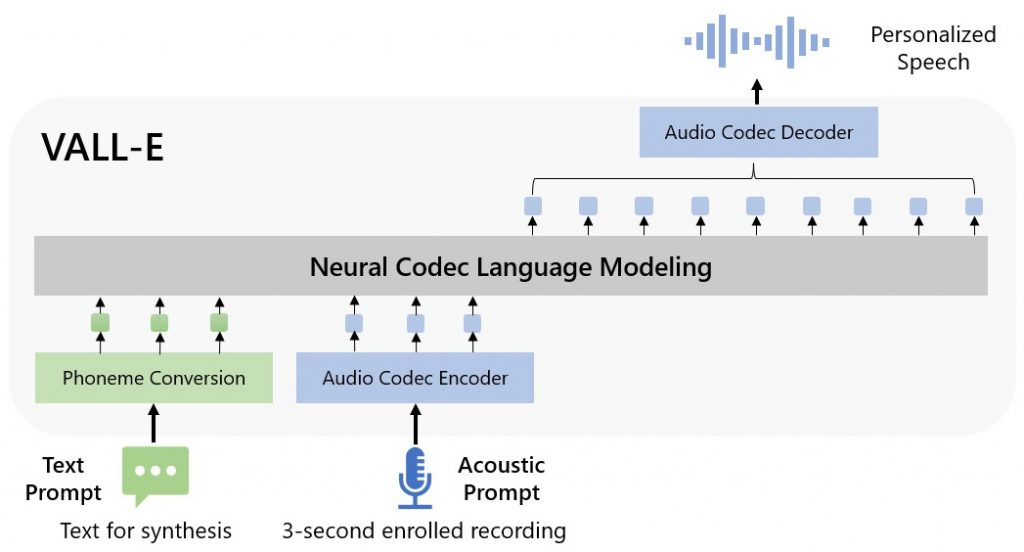
\includegraphics[width=\textwidth]{figures/2-sota/vall-e.jpg}
    \caption[VALL-E]{\textbf{VALL-E} --- The image was extracted from the source publication. It illustrates that both encodings derived from a linguistic prompt and an auditory prompt - provided via the codec encoder - are fed into a language model such as a transformer, and the resulting outputs are passed to the codec decoder to generate audio.}
    \label{fig:vall-e}
\end{figure}

The researchers trained VALL-E using the LibriLight dataset~\cite{kahn_libri-light_2020}, which consists of 60,000 hours of English speech from over 7,000 unique speakers. The proposed approach is robust to noise and generalizes well by leveraging a large and diverse dataset. Previous \ac{TTS} systems are typically trained with fewer data than VALL-E.

VALL-E's performance was evaluated on the LibriSpeech~\cite{panayotov_librispeech_2015} dataset, where all test speakers are unseen during training. VALL-E delivers high performance for speaker-adaptive \ac{TTS} in terms of speech naturalness and speaker similarity, as measured by comparative mean opinion score and similarity mean opinion score, respectively.

Qualitative analysis of VALL-E reveals several interesting findings. Firstly, VALL-E generates speech with diversity. As a result, the same input text can produce different speech outputs. This feature is important for downstream applications such as speech recognition, where diverse inputs with different speakers and acoustic environments are beneficial. The diversity of VALL-E makes it an ideal candidate for generating pseudo-data for speech recognition.

Another finding is that VALL-E maintains the acoustic environment of the prompt during speech synthesis. When the acoustic prompt has reverberation, VALL-E can synthesize speech with reverberation, whereas the baseline outputs clean speech. This can be attributed to VALL-E being trained on a large-scale dataset with diverse acoustic conditions, which allows it to learn acoustic consistency instead of only a clean environment during training.

Furthermore, VALL-E can preserve the emotion in the prompt during speech synthesis. The researchers selected acoustic prompts from the EmoV-DB dataset~\cite{adigwe_emotional_2018}, which contains speech with five emotions. VALL-E kept the exact emotion of the prompt in speech synthesis, even without fine-tuning on an emotional \ac{TTS} dataset.

VALL-E represents a significant advancement in \ac{TTS} technology, with its language model approach and use of audio codec codes as intermediate representations.

In summary, VALL-E is a language model-based \ac{TTS} system that utilizes audio codec codes as intermediate representations. It performs highly in speaker-adaptive \ac{TTS} and demonstrates exciting features such as speech diversity, acoustic environment consistency, and emotion preservation.

\subsubsection{Generative Music}

Generative music is created using generative techniques. End-to-end generative music models enable the production of new musical compositions without using predefined templates or samples, directly from textual or other data inputs. These models use \ac{DL} architectures to capture patterns and structures within different genres or styles of music, and can produce original pieces based on given prompts. This Section explores remarkable generative music models that demonstrate their ability to compose novel musical arrangements.

\paragraph{Jukebox}

Jukebox, a generative model for music that produces music with singing in the raw audio domain, was introduced by Dhariwal et al. in 2020 \cite{dhariwal_jukebox_2020}. The model tackles the long context of raw audio using a multiscale \ac{VQ-VAE} (see Section \ref{sec:ms-vq-vae}) to compress it to discrete codes and models those using \ac{AR} Transformers (see Section \ref{sec:transformers}).

The hierarchical \ac{VQ-VAE} architecture compresses audio into a discrete space, retaining the maximum amount of musical information at increasing compression levels. The model uses residual networks consisting of WaveNet-style (see Section \ref{sec:wavenet}) noncausal 1-D dilated convolutions, interleaved with downsampling and upsampling 1-D convolutions to match different hop lengths. Separate autoencoders with varying hop lengths are trained to maximize the amount of information stored at each level.

After training the \ac{VQ-VAE}, a prior $p(z)$ over the compressed space is learned to generate samples. The prior model is broken up as $p(z) = p(z_{top})p(z_{middle}|z_{top})p(z_{bottom}|z_{middle}, z_{top})$, and separate models are trained for the top-level prior $p(z_{top})$, and upsamplers $p(z_{middle}|z_{top})$ and $p(z_{bottom}|z_{middle}, z_{top})$. Autoregressive Transformers with sparse attention are used for modeling in the discrete token space produced by the \ac{VQ-VAE}.

Jukebox can generate high-fidelity and diverse songs with coherence for up to multiple minutes. It can be conditioned on the artist and genre to steer the musical and vocal style and on unaligned lyrics to make the singing more controllable. The model's release includes thousands of non-cherry-picked samples, model weights, and code.
\paragraph{Riffusion} \label{sec:riffusion}

Riffusion~\cite{forsgren_riffusion_2022} is an open-source model presented in 2022 that generates music clips from text prompts. The model is based on Stable Diffusion (see Section \ref{sec:stable-diffusion}). Riffusion fine-tunes Stable Diffusion to generate images of spectrograms, which can then be converted to music clips.

The authors use \ac{STFT} (see Section \ref{sec:stft}) to compute the spectrogram from audio. The \ac{STFT} is invertible so that the original audio can be reconstructed from a spectrogram. The authors use the Griffin-Lim algorithm~\cite{griffin_signal_1984} to approximate the phase when reconstructing the audio clip.

The authors use diffusion models (see Section \ref{sec:diffusion}) to condition the model's creations on a text prompt and other images, which is helpful for modifying sounds while preserving the structure of an original clip. The authors also use the denoising strength parameter to control how much to deviate from the original clip and towards a new prompt.

So, for inference, the model takes a text prompt as input. Then, the text is encoded into a latent representation using a text encoder. The model generates an image of a spectrogram from the latent representation using a modified version of Stable Diffusion; this is, the Stable Diffusion model fine-tuned for spectrograms. Finally, the generated spectrogram image is converted into an audio clip using the Griffin-Lim algorithm.
\paragraph{MusicLM} \label{sec:musiclm}

MusicLM is a generative model capable of synthesizing high-fidelity music characterized by realistic instrument timbres, accurate pitch, temporal patterns, and smooth transitions between notes based solely on textual descriptions of desired musical attributes (see Section~\ref{sec:musiclm}). The model extends the AudioLM framework for audio generation (see Section~\ref{sec:audiolm}) by incorporating text conditioning via the joint music-text model MuLan (see Section~\ref{sec:mulan}).

MusicLM employs a hierarchical modeling approach with two main stages: semantic modeling and acoustic modeling. The semantic modeling stage uses a Transformer decoder (see Section~\ref{sec:transformers}) to predict semantic tokens from the MuLan audio tokens. Using a separate Transformer decoder, the acoustic modeling stage then predicts acoustic tokens conditioned on both the MuLan audio tokens and predicted semantic tokens. This stage is subdivided into coarse and fine modeling substages to reduce the length of the token sequences, following the AudioLM approach.   

Overall, MusicLM leverages pre-trained audio encoders (SoundStream, w2v-BERT, and  MuLan) to obtain discrete acoustic and semantic tokens as input, after which hierarchical Transformer decoders first predict semantic tokens and then acoustic tokens when conditioned on MuLan text embeddings during synthesis. The hierarchical approach and use of semantic tokens aims to enable coherent long-term generation over extended durations.

MusicLM can generate coherent musical sequences up to 5 minutes in duration, constituting a notable achievement in the context of generative music models. The model captures various musical characteristics specified in textual prompts, including instrument timbre, melodic elements, and musical genre.

The model's performance was assessed using the MusicCaps dataset which comprises 5,500 pairs of music-texts that have been annotated by experts. The dataset includes diverse genres, instruments, and moods. The authors assert that this dataset thoroughly assesses the model's capability to generate various aspects of music from textual prompts. The evaluation metrics comprise human judgments of similarity between the generated outcomes and the prompts, as well as overall quality and others.    

The paper discusses potential limitations, including a proclivity for mode collapse and difficulty generating fine-grained structures over long sequences. However, further investigation is needed to probe the model's limitations and failure modes in greater depth.

In summary, MusicLM represents a promising generative model capable of synthesizing high-fidelity music from textual descriptions via shared embedding spaces and learned associations between text and music encodings, enabling it to capture diverse musical characteristics specified in textual prompts. The MusicCaps dataset provides a valuable means of evaluating the model's performance across various musical styles and prompts.

\subsubsection{General Text-to-Audio}

Text-to-audio systems have a wide range of applications beyond speech synthesis or generative music tasks. End-to-end models convert different forms of textual input into corresponding audio outputs. The outputs have diverse purposes, including sound effects generation, voice transformation, and environmental sound synthesis. These models provide flexible solutions for transforming text into realistic auditory experiences by training on large-scale datasets containing paired text-audio examples across various domains. This Section presents several text-to-audio approaches that demonstrate innovative methods of audio synthesis based on specific textual cues.

\paragraph{SampleRNN} \label{sec:samplernn}

\textit{SampleRNN} is a neural audio generation model proposed in 2017 that can produce high-quality audio samples from scratch \cite{mehri_samplernn_2017}. It uses a hierarchical structure of \acp{RNN} (see Section \ref{sec:rnn}) to model the probability distribution of audio waveforms at different temporal resolutions. The lowest \ac{RNN} operates on individual samples, while higher \acp{RNN} capture longer-term dependencies and structure. SampleRNN can learn from any audio data without any prior knowledge or labels.

The higher \acp{RNN} capture the longer-term dependencies by receiving inputs from lower \acp{RNN} at a lower sampling rate. This way, they can process longer audio sequences. The higher \acp{RNN} also use skip connections to directly access the outputs of lower \acp{RNN}, which helps to avoid vanishing gradients and preserve information across different levels of abstraction.

Each cell is a \ac{RNN} variant, such as \ac{GRU} (see Section \ref{sec:rnn-variants}) that takes as input a frame of audio samples from a lower \ac{RNN} and outputs a hidden state vector that encodes the long-term context of the audio. This output is passed upwards in the hierarchy to other \acp{RNN} that take it. Multiple layers are possible, each operating at a different temporal resolution. All the outputs are then inputted in the final level \ac{RNN}, whose output is the next audio sample based on the combined information from all hierarchy levels.
\paragraph{AudioLM} \label{sec:audiolm}

The framework called AudioLM was introduced by Borsos et al. in 2022 as a means for high-quality audio generation with long-term consistency~\cite{borsos_audiolm_2022}. In this representation space, the framework maps input audio to a sequence of discrete tokens and treats audio generation as a language modeling task. AudioLM achieves high-quality synthesis and long-term structure through a hybrid tokenization scheme. This scheme combines the discretized activations of a masked language model pre-trained on audio (semantic tokens) and the discrete codes produced by a neural audio codec (acoustic tokens).

The AudioLM framework consists of three main components:

\begin{enumerate}
	\item A \textit{tokenizer model} that maps the input audio $x$ into a sequence $y = \text{enc}(x)$ of discrete tokens from a finite vocabulary, with $T' < T$.
	\item A \textit{decoder-only Transformer language model} that operates on the discrete tokens $y$, trained to maximize the likelihood $\prod_{t=1}^{T'} p(y_t|y_{<t})$. The model predicts the token sequence $\hat{y}$ autoregressively at inference time.
	\item A \textit{detokenizer model} that maps the sequence of predicted tokens back to audio, producing the waveform $\hat{x} = \text{dec}(\hat{y})$.
\end{enumerate}

The tokenizer and detokenizer models are pre-trained and frozen before training the language model, simplifying the training setup. The number of tokens $T'$ is significantly smaller than $T$, allowing for increased temporal context size in the language model.

To reconcile the conflicting requirements of high-quality audio reconstruction and capturing long-term dependencies, AudioLM relies on a combination of acoustic and semantic tokens. Acoustic tokens are computed using SoundStream (see Section~\ref{sec:soundstream}). Semantic tokens are computed using w2v-BERT~\cite{chung_w2v-bert_2021}, a model for learning self-supervised audio representations. The semantic tokens enable long-term structural coherence while modeling the acoustic tokens conditioned on the semantic tokens enables high-quality audio synthesis.

AudioLM adopts a hierarchical approach by first modeling the semantic tokens for the entire sequence and then using these as conditioning to predict the acoustic tokens. AudioLM generates syntactically and semantically plausible speech continuations while maintaining speaker identity and prosody for unseen speakers when trained on speech without any transcript or annotation. The approach also extends beyond speech, generating coherent piano music continuations despite being trained without any symbolic representation of music.
\paragraph{DiffSound}

\textit{DiffSound} was presented in a paper, in 2022, that displays a novel text-to-sound generation framework that uses a text encoder, a \ac{VQ-VAE}, a decoder, and a vocoder. The framework takes text as input and outputs synthesized audio corresponding to the input text. The decoder, in particular, is a critical component of the framework, and the paper focuses on designing a suitable decoder, calling it \textit{DiffSound} \cite{yang_diffsound_2022}.

DiffSound is a diffusion decoder (Section \ref{sec:diffusion}) based on the discrete diffusion model. DiffSound predicts all Mel-Spectrogram tokens in one step and then refines the predicted tokens in the next step, resulting in better-predicted results after several steps. It not only produces better text-to-sound generation results compared to an \ac{AR} decoder, but it is also faster, with a generation speed five times faster than an \ac{AR} decoder.

The entire framework acts as this: First, the text is encoded into embeddings using a model like a transformer (Section \ref{sec:transformers}). Then, this representation conditions the generation of spectrogram embeddings using diffusion (the DiffSound model). These embeddings are then passed through the pretrain \ac{VQ-VAE} decoder to generate the spectrogram. The spectrogram runs through a vocoder (Section \ref{sec:vocoders}) to generate the waveform. In the original text, the vocoder used was the MelGAN (see Section \ref{sec:melgan}). This process can be seen in Figure \ref{fig:diffsound}.

\begin{figure}[ht]
    \centering
    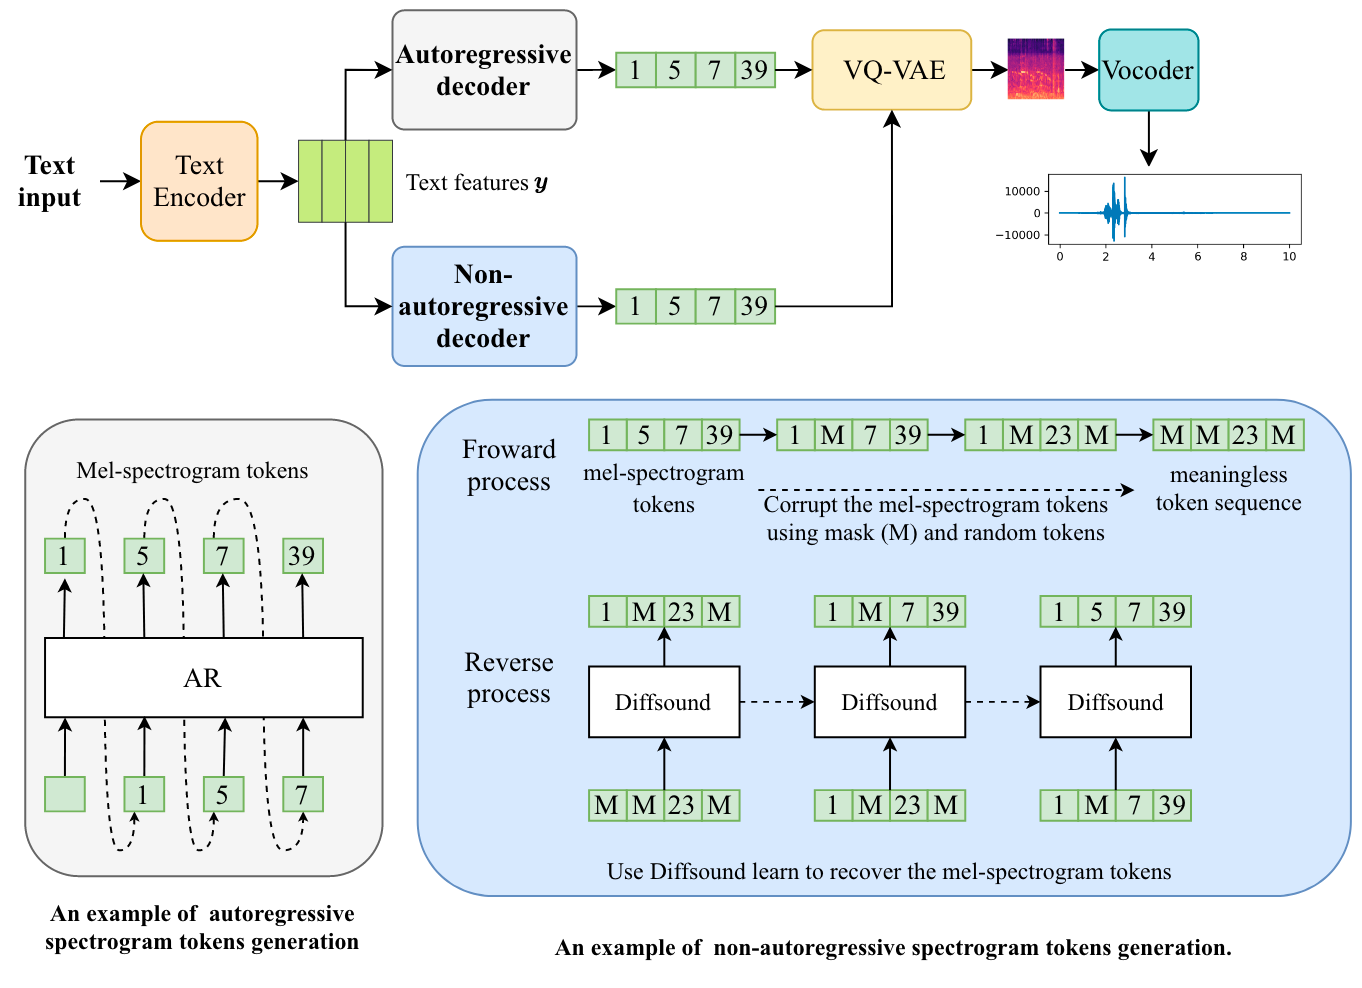
\includegraphics[width=\textwidth]{figures/2-sota/diffsound.png}
    \caption[DiffSound framework]{\textbf{DiffSound framework} --- This illustration was taken from the original paper. At the top, the general framework is present. Two decoders are present, but only one of them is used. The decoder results in a set of latent features. These features are passed to the decoder of the \ac{VQ-VAE} that generates a Mel-Spectrogram (the square with red and blue tones) that, through a vocoder, generates a sound. The two bottom images represent the two decoders. One is a \ac{DARN} (see Section \ref{sec:darn}), the other works with diffusion.}
    \label{fig:diffsound}
\end{figure}
\paragraph{AudioGen} \label{sec:audiogen}

In 2023, Kreuk et al.~\cite{kreuk_audiogen_2023} proposed AudioGen, an auto-regressive generative model that generates audio samples conditioned on text inputs. The model comprises two primary stages: (i) learning a discrete representation of the raw audio using an \ac{AE} method and (ii) training a Transformer language model (see Section~\ref{sec:transformers}) over the learned codes obtained from the audio encoder, conditioned on textual features. During inference, the model samples from the language model generate a new set of audio tokens given text features, which can then be decoded into the waveform domain using the decoder component.

To address the challenge of text-to-audio generation, the authors propose an augmentation technique that mixes different audio samples to train the model to separate multiple sources internally. Furthermore, the authors explore the use of multi-stream modeling for faster inference, allowing the use of shorter sequences while maintaining a similar bitrate and perceptual quality. The proposed method outperforms evaluated baselines over both objective and subjective metrics. Additionally, the authors extend the proposed method to conditional and unconditional audio continuation, demonstrating its ability to generate complex audio compositions.


